\section{Vector spaces and fields}\label{real-and-complex-vector-spaces}
A vector in a vector space is just something which can be added to another vector from the vector
space, and scaled by a scalar from the associated field. A vector does not involve any numbers until
it is represented as a linear combination of basis vectors, using numbers from the associated
field. So whether something is a ``real vector space​'' or a ``complex vector space​'' depends only on
the field. If the field is $\R$ it is a real vector space; if the field is $\C$ it's a complex
vector space. It doesn't make sense to ask whether the vectors themselves are real or complex.

A \defn{field} is a set which is an abelian group under both addition and multiplication.

A \defn{vector space} is an additive abelian group $X$, together with a field $F$, such that $X$ is
closed under linear combinations with scalars from the field $F$.

\subsubsection{Examples}

\begin{enumerate}
\item $\R$ is a field.

\item $\R^2$ is not a field; multiplication is undefined.

\item If we equip $\R^2$ with complex multiplication then this is the field called $\C$.

\item The additive abelian group $\R$, together with the field $\R$, is a one-dimensional vector space.

  {\bf Proof:} Let $x \in \R$ with $x \neq 0$. Then $\{x\}$ is a basis for $\R$, since every element of $\R$ can
  be expressed uniquely as a scalar multiple of $x$. So $\R$ is one-dimensional.

\item The additive abelian group $\R^n$, together with the field $\R$, is a vector space. It is $n$-dimensional.

\item The additive abelian group $\C$, together with the field $\R$, is a two-dimensional vector
  space. It is isomorphic to $\R^2$.

\item The additive abelian group $\C$, together with the field $\C$, is a one-dimensional vector space.

  {\bf Proof:} Let $z \in \C$ with $z \neq 0$. Then $\{z\}$ is a basis for $\C$, therefore $\C$ as a
  complex vector space is one-dimensional.
\end{enumerate}

\newpage
\section{Examples of vector spaces}
\begin{enumerate}
\item The set $\R^n$ of $n-$tuples of real numbers, under componentwise addition and componentwise
  multiplication by real scalars.
\item Complex numbers
  \begin{enumerate}
  \item $\C$ under addition with multiplication by scalars from $\C$ is a field, and therefore a
    vector space. It is one-dimensional ($1$ and $i$ are not linearly independent).
  \item The set $\C^n$ of $n-$tuples of complex numbers, under componentwise addition and
    componentwise multiplication by complex numbers.
  \item $\C$ under addition with multiplication by real scalars is equivalent to $\R^2$.
  \end{enumerate}
\item Matrices \& linear transformations:
  \begin{enumerate}
  \item The set $M_{m \times n}(\R)$ of $m\times n$ matrices is a vector space, under componentwise
    addition and multiplication by real scalars.
  \item The set $\mathrm{Hom}(V, W)$ of linear transformations from vector space $V$ to vector
    space $W$ is a vector space: for scalar $a$, define $(aT)(v) := a(T(v))$, and
    $(S + T)v := S(v) + T(v)$.
  \end{enumerate}
\item The set $\R_n[x]$ of polynomials of degree $\leq n$ is a real vector
  space.
\item The set $\R^X$ of real-valued functions on any set $X$ is a real vector
  space. Examples:
  \begin{enumerate}
  \item Let $[n] = \{1, 2, \ldots, n\}$. Note that the function space $\R^{[n]}$ is
    the same as $\R^n$ (both are sets of $n-$tuples of reals).
  \item Similarly, $\R^{[m]\times[n]}$ is the same as $M_{m \times n}(\R)$.
  \item $\R^\R$, the set of all functions $\R\to\R$.
  \item The set of continuous functions $\R \to \R$, and differentiable functions
    $\R \to \R$, under pointwise addition and pointwise scalar multiplication
    (from any field?).
  \item Set of solutions of a homogeneous linear ODE
  \end{enumerate}
\item Sequences $(a_n)$ of real numbers, under term-wise addition and term-wise
  scalar multiplication, form a vector space, identifiable with the function
  space $\R^\N$. Examples:
  \begin{enumerate}
  \item Set of convergent sequences
  \end{enumerate}
\item The set of solutions of a system of \textit{homogeneous} linear equations
  in $n$ variables is a subspace $V$ of $\R^n$. (Let $A$ be the matrix
  representing the system and let $u$ and $v$ be solutions. Then $Au = Av = 0$
  and $V$ is a subspace since $A(u + v) = Au + Av = 0$, and
  $A(\lambda u) = \lambda Au = 0$.)
\end{enumerate}

\section{Linear systems}

Consider the linear systems
\begin{align*}
  \begin{array}{cc}
    \begin{cases}
      x = 0\\
      y = 0
    \end{cases}
    ~~~~~~~~~~~~~~~~~~~~~~~~~~~~&
    \begin{cases}
      x - y = 0\\
      x + y = 1\\
      x - z = 0
    \end{cases}
  \end{array}
\end{align*}

A ``solution'' is an assignment of values to the $n$ variables which makes all
$m$ equations true.

In other words, we notice that the equations involve $n$ variables, and
consider the set of $n$-tuples
$S = \{(x, y, \ldots) ~|~ x, y, \ldots \in  \R\}$.

The set of solutions is the subset of $S$ for which all the equations are true.

Geometrically, we think of the 2-tuple $(a, b)$ as a point in the $\R^2$
plane. Specifically, if our basis is $\vec e_1, \vec e_2$, then $(a, b)$ is the
point $a\vec e_1 + b\vec e_2$. We might imagine that the basis is the standard
orthogonal basis, but that's not necessary.

The linear equations define hyperplanes (lines, planes etc) in $S$.

The set of solutions is the intersection of these hyperplanes: another
hyperplane or the empty set.

So at this point, we do not treat the ambient space as a vector space (we're
not adding or scaling points), and neither the equation hyperplanes nor the
solution hyperplane, need be a subspace (since it need not contain the origin).

Next, we rewrite the linear system as a matrix applied to a vector, $Ax = b$:
\begin{align*}
  \begin{array}{cc}
    \matMMxNN{1}{0}
        {0}{1} \vecMM{x}{y} = \vecMM{0}{0}
    ~~~~~~~~~~~~~~~~~~~~~~~~~~~~~~~~~~~~~~~&
    \matMMMxNN{1}{-1}
              {1}{~~1}
              {1}{-1} \vecMM{x}{y} = \vecMMM{0}{1}{0}.
  \end{array}
\end{align*}

The equation coefficients are now represented by a linear transformation
$A:\R^n \to \R^m$.

This matrix equation is saying:
\begin{enumerate}
\item Let the $x$ coefficients be a vector $\vec a_1 \in  \R^m$. And let the $y$
  coefficients be another vector $\vec a_2 \in  \R^m$, and so on.
\item So now you have $n$ vectors spanning some subspace of $\R^m$.
\item Is $b$ in their span? If so, for what values of $x, y, \ldots$ does
  $x\vec a_1 + y\vec a_2 + \cdots = b$?
\end{enumerate}

From Frenkel's Multivariable Calculus lectures:

\begin{center}
  \begin{quote}
    \textit{The dimensionality of an object is equal to the dimensionality of the
      ambient space, minus the number of independent equations.}
  \end{quote}
\end{center}

So, basically, suppose there are $n$ variables. Then the solution set is a
subset (hyperplane) of $\R^n$, and

\begin{tabular}{c|c}
  Independent equations & Solution set\\
  \hline
  1                     & $(n - 1)$-dimensional hyperplane \\
  2                     & $(n - 2)$-dimensional hyperplane \\
  \vdots                & \vdots \\
  $n-1$                 & line \\
  $n$                   & point \\
  $n + 1$               & impossible \\
  \vdots                & \vdots
\end{tabular}

So when do we get no solutions? That's when
\begin{align*}
  &\text{the $n$ columns of $A$ do not span $\R^m$}\\
  \iff &\Rank A < \text{(number of equations)}\\
  \iff &\text{not all equations independent},
\end{align*}
and $b$ is not in their span.

In other words, suppose we have a linear system involving $n$ variables.

Suppose that all the $m$ equations are independent: full row rank.

Then $m \leq n$.

Now we introduce a dependent equation into the system.

\red{One error above is that its only the coefficients of the equation that
  we're considering when we say the rows are dependent/independent. So it's not
  correct to talk about ``independent equations''.}


\section{Subspaces}
A subspace $U$ of $V$ is a subset of $V$ for which
\begin{enumerate}
\item $0 \in  U$
\item For any finite subset $U^* \subset U$, the set of all linear combinations
  of $U^*$ is also a subset of $U$.
\end{enumerate}

\section{Span, basis, dimension}
\begin{theorem}
  Every basis has the same size.
\end{theorem}

\begin{proof} Let $v_1, \ldots, v_n$ be a basis for a vector space $V$.


\end{proof}

\begin{theorem}
  A spanning set that is the same size as a basis is also a basis.
\end{theorem}

\begin{proof}
  Let $v_1, \ldots, v_n$ be a basis for a vector space $V$, and let
  $u_1, \ldots, u_n$ span $V$.

  We know that $v_1, \ldots, v_n$ are linearly independent and that if we
  remove any one of them they will cease to span.

  We want to show that $u_1, \ldots, u_n$ are linearly independent.

  Suppose, that the $u_i$ are not linearly independent and that
  $u_2, \ldots, u_n$ span $V$. Thus there are $n-1$ vectors in this spanning
  set. But the Steinitz Exchange Lemma states that if $v_1, \ldots, v_n$ are
  linearly independent and $u_1, \ldots, u_m$ span, then $n \leq m$. This
  contradiction proves that the $u_i$ are linearly independent.
\end{proof}

\begin{theorem}\label{transformed-basis-is-a-basis}
  Let $U, V$ be vector spaces, let $f:U \to  V$ be an invertible linear map, and let
  $e_1, \ldots, e_n$ be a basis for $U$. Then $f(e_1), \ldots, f(e_n)$ is a basis for $V$.
\end{theorem}

\begin{proof}We need to show that the $f(e_i)$ are linearly independent and spanning.

  \begin{enumerate}
  \item {\bf Linear independence}\\
    Suppose $\sumin \lambda_if(e_i) = 0$.

    Therefore $f\(\sumin \lambda_ie_i\) = 0$ since $f$ is linear.

    Therefore $\sumin \lambda_ie_i = f^\1(0) = 0$, since the preimage of $0$ is $\{0\}$ for an
    invertible linear map.

    But the $e_i$ are linearly independent, therefore $\lambda_i = 0$ for all $i = 1, \ldots n$, as
    required.

  \item {\bf Spanning}\\
    Let $v \in V$.

    Then $v = f(u)$ for some $u \in  U$, since $f$ is surjective.

    Therefore $v = f\(\sumin \lambda_ie_i\) = \sumin \lambda_if(e_i)$ for some
    $\lambda_1, \ldots, \lambda_n$, as required.

  \end{enumerate}
\end{proof}

\begin{problem*}
  If $u, v$ are linearly independent under one basis are they linearly independent under all choices of basis?
\end{problem*}

\section{Linear transformations and matrices}

A linear transformation is completely specified by

\begin{enumerate}
\item Some basis vectors $i$ and $j$
\item Where those basis vectors are taken to by the transformation.
\end{enumerate}

How the transformation affects any other point follows from those two pieces of
information.

So $i$ might be taken to $ai + bj$, and $j$ might be taken to $ci + dj$.
In this case we would use the following matrix to describe the
transformation:

$$
\matMMxNN{a}{c}
    {b}{d}
$$

Some examples are

$$
\begin{array}{ll}
\text{stretch by a in the i-direction} & \matMMxNN{a}{0}
                                             {0}{1}
\\\\
\text{stretch by a in the i-direction and shear right} & \matMMxNN{a}{b}
                                                             {0}{1}
\\\\
\text{rotate anticlockwise 90°} & \matMMxNN{0}{-1}
                                      {1}{ 0}
\end{array}
$$

Note that we haven't said what $i$ and $j$ are yet; they \textit{define} the
2-dimensional space that we're considering. But, we can think of them for now
as the usual orthogonal unit vectors in 2D space.

So the matrix tells us where the basis vectors have been taken to. Any other
vector $fi + gj$ is taken to wherever that is using the transformed basis
vectors:

$$
fi + gj \longrightarrow f\cvec{a}{b} + g\cvec{c}{d} = \cvec{fa + gc}{fb + gd}
$$


And that's how matrix multiplication is defined:

$$
\matMMxNN{a}{c}
    {b}{d} \cvec{f}{g} = \cvec{fa + gc}{fb + gd}
$$


A matrix represents a linear transformation by showing where the basis vector
are taken to.

\begin{theorem}
  The inverse of a 2x2 matrix is
  \begin{align*}
   \matMMxNN{a}{c}
       {b}{d}^{-1}
  =
  \frac{1}{\text{det}} \matMMxNN{d }{-c}
                           {-b}{a}
  \end{align*}
  where $\text{det} = ad - cb$.
\end{theorem}

\section{Geometric interpretation of matrix operations}
\url{https://math.stackexchange.com/questions/37398/what-is-the-geometric-interpretation-of-the-transpose}
\url{https://math.stackexchange.com/questions/598258/determinant-of-transpose/636198#636198}


\section{Commutativity}
\subsection{Examples of transformations that don't commute}
Let $A$ be reflection around the first coordinate axis $\matMMxNN{1}{0}
                                                                 {0}{-1}$
and let $B$ be $90\deg$ anticlockwise rotation $\matMMxNN{0}{-1}
                                                         {1}{0}$.

Then $BA = \matMMxNN{0}{1}
                    {1}{0}
\neq  AB = \matMMxNN{0}{-1}
                    {-1}{0}$.

Note that $A^\1 = A = A^T$ and $B^\1 = \matMMxNN{0}{1}
                                               {-1}{0} = B^T$.

Therefore these are both orthogonal (unitary) matrices.


\section{Eigenvalues, eigenvectors, characteristic polynomial}

Let $V$ be a vector space and let $T:V \to V$ be a linear transformation.

\begin{definition*}[eigenvalue]
  $\lambda$ is an \textit{eigenvalue} of $T$ iff there exists \todo{non-zero?} $v \in V$ such that
  $Tv = \lambda v$.
\end{definition*}

\begin{definition*}[eigenspace]
  $E_\lambda = \{v ~|~ Tv = \lambda v\}$ is an \textit{eigenspace} of $T$.
\end{definition*}

\begin{definition*}[eigenvector]
  An \textit{eigenvector} is a non-zero element of an eigenspace.
\end{definition*}

\begin{definition*}[characteristic polynomial]
  The characteristic polynomial of $T$ is $\chi_T(x) = \det(T - xI)$. Note that
  $\lambda$ is an eigenvalue of $T$ iff $x=\lambda$ is a root of $\chi_T(x)$.
\end{definition*}

\begin{intuition*}~\\
  Decompose $T$ as the sum of two transformations: $T = \lambda I + T^*$. This
  means that the effect of applying $T$ to a vector is the same as applying
  $\lambda I$ to the vector, and separately applying $T^*$ to the same vector,
  and adding the two results.

  Note that applying $\lambda I$ to a vector just scales the vector by $\lambda$.

  Note that $T^* = T - \lambda I$.

  Therefore what $T - \lambda I$ does to a vector is: whatever remains to be done after
  scaling by $\lambda$, in order to have the same effect as $T$.

  Suppose $\lambda$ is an eigenvalue. Then there exists an eigenspace
  $E_\lambda$ (a line, at least) containing vectors which are simply stretched
  by a factor $\lambda$. So for $v \in E_\lambda$, nothing remains to be done
  after scaling by $\lambda$, and so we have $(T - \lambda I)(v) = 0$.

  Therefore
  \begin{itemize}
  \item If $T - \lambda I$ has a nullspace containing a non-zero element, then
    $\lambda$ is an eigenvalue and the nullspace is the eigenspace for
    $\lambda$.
  \item The roots of $\det(T - xI)$ are the eigenvalues of $T$.
  \end{itemize}

\end{intuition*}

\begin{remark*}[Repeated eigenvalues]~\\
  If two eigenvectors share the same eigenvalue then they are in the same eigenspace.
\end{remark*}

\begin{proof}
  Suppose that $Tv_1 = \lambda v_1$ and $Tv_2 = \lambda v_2$ and
  $v_1 \neq v_2$, and let $a$ be a scalar.

  Then
  $T(v_1 + av_2) = T(v_1) + aT(v_2) = \lambda v_1 + a\lambda v_2 = \lambda(v_1
  + av_2)$.
\end{proof}



\begin{example*}
  $A = \mat
  {0}{-1}
  {1}{0}$ is a rotation anticlockwise by $90\deg$. So it should be found to not
  have any eigenvectors.

  So let's try to find the eigenvectors. The eigenvalues of $A$ are the solutions to
  $\det (A - \lambda I) = 1 -\lambda^2 = 0$, so $\lambda = 1, -1$.

  If $\lambda = 1$ then we have
  \begin{align*}
    \matMMxNN{0}{-1}{1}{0}\pvecc{x_1}{x_2} &= \pvecc{x_1}{x_2} \\
    \pvecc{-x_2}{x_1} &= \pvecc{x_1}{x_2},
  \end{align*}
  and if $\lambda = -1$ then we have
  \begin{align*}
    \matMMxNN{0}{-1}{1}{0}\pvecc{x_1}{x_2} &= \pvecc{-x_1}{-x_2} \\
    \pvecc{-x_2}{x_1} &= \pvecc{-x_1}{-x_2},
  \end{align*}
  so that $\pvecc{x_1}{x_2} = \pvecc{0}{0}$ is the only solution in both cases.
\end{example*}

\begin{example*}
  $A = \mat {\cos \theta}{-\sin \theta} {\sin \theta}{\cos \theta}$ is a rotation anticlockwise by
  $\theta \deg$. So it should be found to not have any eigenvectors.

  So let's try to find the eigenvectors. The eigenvalues of $A$ are the solutions to
  \begin{align*}
    \det (A - \lambda I)
    &= (\cos\theta - \lambda)^2 + \sin^2\theta \\
    &= \lambda^2 - 2\lambda\cos\theta + 1 \\
    &= 0,
  \end{align*}
  so that
  \begin{align*}
    \lambda
    &= \frac{2\cos\theta \pm \sqrt{4\cos^2\theta - 4}}{2} \\
    &= \cos\theta \pm \sqrt{\cos^2\theta - 1} \\
    &= \cos\theta \pm \sin\theta.
  \end{align*}

  If $\lambda = \cos\theta + \sin\theta$ then we have
  \begin{align*}
    \mat
    {\cos \theta}{-\sin \theta}
    {\sin \theta}{\cos \theta} \pvecc{x_1}{x_2}
    &= \pvecc{(\cos\theta + \sin\theta)x_1}{(\cos\theta + \sin\theta)x_2} \\
    \pvecc{x_1\cos\theta - x_2\sin\theta}{x_1\sin\theta + x_2\cos\theta}
    &= \pvecc{(\cos\theta + \sin\theta)x_1}{(\cos\theta + \sin\theta)x_2} \\
    \begin{cases}
      x_1\sin\theta = -x_2\sin\theta \\
      x_1\sin\theta = x_2\sin\theta.
    \end{cases} \\
    \begin{cases}
      \sin\theta(x_1 + x_2) = 0 \\
      \sin\theta(x_1 - x_2) = 0,
    \end{cases}
  \end{align*}
  so either $\theta = 2\pi k$ or $\pvecc{x_1}{x_2} = 0$, as expected.

\end{example*}



\section{Change of basis}

Suppose person B uses some other basis vectors to describe locations in
space. Specifically, in our coordinates, their basis vectors are
$\scvec{2}{1}$ and $\scvec{-1}{1}$.


\textbf{When they state a vector, what is it in our coordinates?}

If they say $\scvec{-1}{2}$, what is that in our coordinates?

Well, if they say $\scvec{1}{0}$, that's $\scvec{2}{1}$ in our coordinates. And
if they say $\scvec{0}{1}$, that's $\scvec{-1}{1}$ in our coordinates. So the
matrix containing \textit{their basis vectors expressed using our coordinate system}
transforms a point expressed in their coordinate system into one expressed in
ours. That last sentence is critical, so hopefully it makes sense! So, the answer is

$$
\matMMxNN{2}{-1}
    {1}{ 1} \cvec{-1}{2} = \cvec{-4}{1}.
$$


\textbf{When we state a vector, what is it in their coordinates?}

We give the vector $\scvec{3}{2}$. What is that in their coordinate system? By
definition, the answer is the weights that scales their basis vectors to hit
$\scvec{3}{2}$. So, the solution to

$$
\matMMxNN{2}{-1}
    {1}{1} \cvec{a}{b} = \cvec{3}{2}.
$$


Computationally, we can see that we can get the solution by multiplying both
sides by the inverse:

$$
\cvec{a}{b} = \matMMxNN{2}{-1}
                  {1}{1}^{-1} \cvec{3}{2}.
$$

Conceptually, we have

$$
\matMMxNN{2}{-1}
    {1}{1} =
\begin{pmatrix}\text{matrix converting their}\\\text{representation to ours} \\ \end{pmatrix}
$$

where ``their representation'' means the vector expressed using their coordinate
system. So the role played by the inverse is

$$
\cvec{a}{b} =
\begin{pmatrix}\text{matrix converting our}\\\text{representation to theirs} \\ \end{pmatrix}
\cvec{3}{2}.
$$

\textbf{When we state a transformation, what is it in their coordinates?}

We state a 90° anticlockwise rotation of 2D space:

$$
\matMMxNN{0}{-1}
    {1}{0}
$$

what is that transformation in their coordinates? The answer is

$$
\begin{pmatrix}\text{matrix converting our}\\\text{representation to theirs} \\ \end{pmatrix}
\matMMxNN{0}{-1}
    {1}{0}
\begin{pmatrix}\text{matrix converting their}\\\text{representation to ours} \\ \end{pmatrix}
$$

since the composition of those three transformations defines a single
transformation that takes in a vector expressed in their coordinate system,
converts it to our coordinate system, transforms it as requested, and then
converts back to theirs.

Let
\begin{align*}
  P = \matMMxNN{2}{-1}
          {1}{1}
\end{align*}
be the change-of-basis matrix . Then the matrix, in their coordinates, of the
rotation transformation is
$$
P^\1\matMMxNN{0}{-1}
        {1}{0} P.
$$

What about the uniform stretch transformation? In our coordinates this has
matrix $\lambda I = \matMMxNN{\lambda}{0}
                        {0}{\lambda}$. In their coordinates, it has matrix
\begin{align*}
P^\1\lambda I P = \lambda P^\1 P = \lambda I.
\end{align*}
I.e. a uniform stretch transformation represented by a diagonal matrix has the
same matrix in any basis. That's because -- forget about introducing any basis
-- there is only one ``uniform stretch transformation'': it's the
transformation that acts on space like it's a balloon being inflated
uniformly. Whatever basis vectors you choose, each one $\vec e_i$ is going to be taken
to $\lambda \vec e_i$. That means the matrix of the transformation, in whatever basis,
is $\matMMxNN{\lambda}{0}
        {0}{\lambda}$, because the vector
\begin{quote}
``one unit in the $\vec e_1$ direction, zero units in the $\vec e_2$ direction''
\end{quote}
is going to be taken to the vector
\begin{quote}
``$\lambda$ units in the $\vec e_1$ direction, zero units in the $\vec e_2$ direction''.
\end{quote}

What about a non-uniform stretch transformation?

\newpage
Consider $\R^2$. Fix a first basis vector $e_1$.

Consider the map $T:\R^2\to\R^2$ which stretches space by a factor of 2 in the
direction of $e_1$, and by a factor of 3 in the orthogonal direction.

Suppose that the second basis vector $e_2$ is orthogonal to $e_1$ and has the
same magnitude.

Then the matrix of $T$ is $\matMMxNN{2}{0}
                               {0}{3}$ with respect to this basis.
~\\

Now consider an alternative basis $\{f_1, f_2\}$ where $f_2$ intersects with
$f_1$ at $45\deg$.

Specifically, with respect to basis $\{e_1, e_2\}$, we have $f_1 = (1, 0)$ and
$f_2 = (1, 1)$.

Then the matrix of $T$ with respect to basis $\{f_1, f_2\}$ is
\begin{align*}
  \matMMxNN{1}{1}
      {0}{1}^\1 \matMMxNN{2}{0}
                    {0}{3} \matMMxNN{1}{1}
                               {0}{1} &=
  % \matMMxNN{1}{-1}
  %     {0}{1} \matMMxNN{2}{0}
  %                {0}{3} \matMMxNN{1}{1}
  %                           {0}{1} \\ &=
  \matMMxNN{1}{-1}
      {0}{1}  \matMMxNN{2}{2}
                  {0}{3} \\ &=
  \matMMxNN{2}{-1}
      {0}{3}.
\end{align*}
(It's obvious that $f_1 \mapsto (2, 0)$; that $f_2 \mapsto (-1, 3)$ is clear in
a diagram.)

The eigenvalues of $T$ are clearly 2 and 3, independent of basis.

The eigenspaces are the line through $e_1$, and the line through $e_2$.

So with respect to basis $\{e_1, e_2\}$, the eigenspaces are
$\{(a, 0) ~|~ a \in \R\}$ and $\{(0, a) ~|~ a \in \R\}$.

And with respect to basis $\{f_1, f_2\}$, the eigenspaces are
$\{(a, 0) ~|~ a \in \R\}$ and $\{(-a, a) ~|~ a \in \R\}$.

  % The characteristic polynomial is $\det(A - \lambda I) = 0$, where $A$ is a
  % matrix of $T$ with respect to some basis. Let $A = \matMMxNN{2}{0}
  % {0}{3}$. Then
  % \begin{align*}
  %   \det(A - \lambda I) = \det \matMMxNN{2 - \lambda}{0}
  %   {0}{3 - \lambda} = (2 - \lambda)(3 - \lambda).
  % \end{align*}
  % So the eigenvalues are 2 and 3.

  % The eigenspace $E_2$ with respect to basis $\{e_1, e_2\}$ is the set of
  % solutions to
  % \begin{align*}
  %   \matMMxNN{2}{0}
  %   {0}{3} \vecMM{x}{y} = \vecMM{2x}{2y}.
  % \end{align*}

\newpage
Consider the map which stretches space by a factor of 2 in one direction, and a
factor of 3 in another direction.

Then there exists a basis for which the map has matrix
$
\matMMxNN{2}{0}
    {0}{3}
$.

What are the eigenspaces of this map?

The characteristic polynomial (basis independent) is $\det(A - \lambda I) = 0$
where $A$ is the matrix of the map wrt some basis.


\subsection{Equation of a line under a change of basis} \label{equation-of-line-under-change-of-basis}
\begin{question*}
  How does the equation of a line change when the basis is changed?
\end{question*}

\begin{proof}
  A straight line in a real vector space $V$ is a set defined by two points $v_1, v_2 \in V$:
  \begin{align*}
    L = \{v_1 + \alpha(v_2 - v_1) ~|~ \alpha \in \R \}.
  \end{align*}
  Equivalently, we can write a ``parametric equation'' for the straight line:
  \begin{align*}
    v(\alpha) = v_1 + \alpha(v_2 - v_1).
  \end{align*}
  This is a map $\R \to L$, i.e. it maps a value of the parameter $\alpha$ to a point on the line.

  Suppose $V = \R^2$ and we specify a basis such that $y = mx + y_0$. Now fix $x_1 \in \R$ and we
  have a parametric equation
  \begin{align*}
    \vecMM{x}{y} &= \vecMM{0}{y_0} + \alpha\vecMM{x_1}{mx_1}.
  \end{align*}

  Now, let $A = \matMMxNN{a_1}{a_2} {a_3}{a_4}$ be the matrix containing the new basis vectors
  (expressed in the original basis). Then with coordinates expressed in the new basis we have
  \begin{align*}
    \vecMM{x}{y}                    &= A^{-1}\vecMM{0}{y_0} + \alpha A^{-1}\vecMM{x_1}{mx_1} \\
    \matMMxNN{a_1}{a_2}
             {a_3}{a_4}\vecMM{x}{y} &= \vecMM{\alpha x_1}{y_0 + \alpha mx_1} \\
    \alpha &= \frac{a_1x + a_2y}{x_1} \\
    a_3x + a_4y &= y_0 + \frac{a_1x + a_2y}{x_1} mx_1 \\
                &= y_0 + a_1mx + a_2my \\
    y &= \frac{a_1m - a_3}{a_4 - a_2m}x + \frac{y_0}{a_4 - a_2m}.
  \end{align*}
\end{proof}

\begin{example*}~\\
  \begin{enumerate}
  \item If the line is a subspace of $\R^2$ (passes through the origin), then
    \begin{align*}
      y = \frac{a_1m - a_3}{a_4 - a_2m}x
    \end{align*}
  \item If the new basis vectors point in the same direction as the original basis vectors, then
    $a_2 = a_3 = 0$ and
    \begin{align*}
      y = \frac{a_1m}{a_4}x + \frac{y_0}{a_4}
    \end{align*}
  \end{enumerate}
\end{example*}
\newpage
\section{Symmetric matrices}

\textbf{Spectral theorem for symmetric matrices}

Symmetric $n \by n$ matrix $A$ (real).

$A^\1 = A^\T$

$n$ orthogonal eigenvectors with real eigenvalues.

Orthonormal matrix $U$ containing normalized eigenvectors.

$A = U\Lambda U^\1 = U\Lambda U^\T$

(Eigenvalues are uniquely determined by matrix. Eigenvalues can be repeated, in which case any linear combination of their
eigenvalues is also an eigenvalue.)

\section{Inner Product Spaces}

Note that if $f(\cdot)$ is linear:
\begin{enumerate}
\item $f(ax + by) = f(ax) + f(by)$.
\end{enumerate}

\begin{definition*}[Bilinear form]~\\
  A bilinear form is a binary function $f(\cdot, \cdot)$ such that:
  \begin{enumerate}
  \item $f(ax + by, z) = f(ax, z) + f(by, z)$
  \item $f(z, ax + by) = f(z, ax) + f(z, by)$.
  \end{enumerate}
\end{definition*}


\begin{claim*}
  The dot product in $\F^n$ is bilinear.
\end{claim*}

\begin{proof}
  \begin{align*}
    \langle ax + by , z \rangle :=& \sum_i (ax + by)_iz_i\\
                                 =& \sum_i (ax_i + by_i)z_i\\
                                 =& \sum_i ax_iz_i + \sum_i by_iz_i\\
                                 =& \langle ax, z \rangle + \langle by, z \rangle\\
    \langle z, ax + by \rangle  :=& \ldots
  \end{align*}
\end{proof}

Note that $\langle x, y \rangle = x \cdot y = x^Ty = x^TIy$.

And note that the ``quadratic form'' $ax^2 + 2bxy + cy^2$ can be written as
\begin{align*}
\x^\T A \x = \cvec{x}{y}^\T \matMMxNN{a}{b}
                                {b}{c} \cvec{x}{y}.
\end{align*}
This is a scalar. In general, a quadratic form for symmetric matric $A$ is
\begin{align*}
\x^\T A \y = \sum_{jk}A_{jk}x_jy_k.
\end{align*}

These quadratic forms are also bilinear forms: the dot product is a quadratic form using the
identity matrix.

\begin{definition*}[Gram matrix]
  Take a collection of vectors $v_1, \ldots, v_n$. A Gram matrix is the $n \times n$ matrix
  $(\langle v_i, v_j \rangle)$.
\end{definition*}

\begin{theorem*}
  Every bilinear form is of the form $\langle u, v \rangle = u^TAv$ for some Gram matrix.
\end{theorem*}

\begin{definition*}
  A bilinear form is symmetric if $\langle u, v \rangle = \langle v, u \rangle$.
\end{definition*}

\begin{theorem*}
  The bilinear form $\langle u, v \rangle := u^TAv$ is symmetric if and only if $A$ is symmetric.
\end{theorem*}

\begin{definition*}
  A \red{TODO (real?)} bilinear form is positive definite if $\langle u, v \rangle > 0$ for all
  $v \in V \setminus \{0\}$. \red{TODO that doesn't make sense}
\end{definition*}

\begin{definition*}[Inner product]~\\
  An inner product is a bilinear form that is symmetric and positive definite.

  An inner product space is a vector space equipped with an inner product.

  In an abstract inner product space we define the angle between $u$ and $v$ to be
  $\cos^\1\Big(\frac{\langle u, v \rangle}{\norm{u}\norm{v}}\Big)$.

  In a real inner product space we define the norm to be $\norm{u} := \sqrt{\langle u, u \rangle}$.
\end{definition*}

\begin{theorem*}[Cauchy-Schwartz inequality]~\\
  Let $V$ be an inner product space and let $u, v \in V$. Then
  $\langle u, v \rangle \leq \norm{u} \norm{v}$.
\end{theorem*}

\begin{proof}
  \red{Are we assuming the inner product is real-valued here?}
  Define $f(t) := \langle tu + v, tu + v \rangle = \norm{tu +v}^2$.

  Use bilinearity and symmetry to show that
  $f(t) = t^2 \langle u, u \rangle + 2t \langle u, v \rangle + \langle v, v \rangle$. (How?)

  The Cauchy-Schwartz inequality follows by noting that the determinant of this quadratic must be
  negative.
\end{proof}

\section{Complex vector spaces}
When viewed as a real vector space (i.e. with real scalars), $\C$ is
two-dimensional, e.g. $\{1, i\}$ is a basis.

When viewed as a complex vector space (i.e. with complex scalars), $\C$ is one-dimensional: $\{1\}$
is a basis; $\{1, i\}$ are no longer linearly independent.

\footnotetext{
  \href{https://www.youtube.com/playlist?list=PLZHQObOWTQDPD3MizzM2xVFitgF8hE_ab}{Essence of Linear Algebra} video series by \href{http://www.3blue1brown.com/}{Grant Sanderson / 3blue1brown}
}

\begin{definition*}
  Let $V$ be a complex vector space.

  $\langle \cdot, \cdot \rangle:V \times V \to \C$ is a sesquilinear form if
  \begin{enumerate}
  \item $\langle au + bv, z \rangle = a\langle u, z \rangle + b\langle v, z \rangle$
  \item $\bar{\langle u, u \rangle} = \langle u, u \rangle$ (therefore
    $\langle u, u \rangle \in \R$).
  \end{enumerate}
\end{definition*}


\begin{definition*}[Hermitian space]~\\
  Let $V$ be a complex vector space (i.e. complex scalars).

  A Hermitian form is a sesquilinear form that is symmetric and positive definite.

  A complex inner product space, or Hermitian space, is a complex space equipped with a Hermitian
  form as an inner product.
\end{definition*}

\section{Computing the n-th Fibonacci number: generating function}

\begin{definition}
  The Fibonacci sequence is defined by $f_0 = f_1 = 1$ and $f_n = f_{n-2} + f_{n-1}$:
  \begin{align*}
    f_0 &= 1\\
    f_1 &= 1\\
    f_2 &= 2\\
    f_3 &= 3\\
    f_4 &= 5\\
    f_5 &= 8\\
    &\ldots.
  \end{align*}
\end{definition}

Our aim is to find a formula for the $n$-th Fibonacci number $f_n$. Some proofs follow below.


\begin{definition}
  The ``golden ratio​'' is $\varphi = \frac{1}{2}(1 + \sqrt 5)$.

  Also define $\psi = 1 - \varphi = \frac{1}{2}(1 - \sqrt 5)$.
\end{definition}

Note that $\varphi^2 = 1 + \varphi$ and $\psi^2 = 1 + \psi$. It follows that for both $\varphi$ and
$\psi$, the $n$-th powers are related to the $(n-1)$-th and $n$-th Fibonacci numbers:
  \begin{align*}
    \varphi^2  &= 1 + \varphi \\
    \varphi^3  &= \varphi + \varphi^2 = 1 + 2\varphi \\
    \varphi^4 &= \varphi + 2\varphi^2 = 2 + 3\varphi \\
    \varphi^5 &= 2\varphi + 3\varphi^2 = 3 + 5\varphi \\
    \varphi^6 &= 3\varphi + 5\varphi^2 = 5 + 8\varphi \\
    \vdots
  \end{align*}

\begin{claim}
  The $n$-th Fibonacci number is given by
  \begin{align*}
    f_n = \frac{1}{\sqrt5}(\varphi^n - \psi^n).
  \end{align*}
\end{claim}

\begin{proof}
  We have (lemma proved below)
\begin{align*}
  \varphi^n &= f_{n-1} + f_n\varphi \\
  \psi^n &= f_{n-1} + f_n\psi.
\end{align*}
  Note also that $\varphi - \psi = 2\varphi - 1 = \sqrt 5$. Therefore $\varphi^n - \psi^n = f_n(\varphi - \psi) = f_n\sqrt5$.
\end{proof}

\begin{lemma}
  \begin{align*}
  \varphi^n &= f_{n-1} + f_n\varphi \\
  \psi^n &= f_{n-1} + f_n\psi.
\end{align*}
\end{claim}

\begin{proof}
  If we define $f_0 = 0$ then the $\varphi$ claim is true for $n=1$ ($\varphi^1 = 0 + 1\varphi$). It's also true for $n=2$ ($\varphi^2 = 1  + 1\varphi$).

  Suppose it's true for $n=k$. Then it's true for $n = k+1$ since
  \begin{align*}
    \varphi^{k+1} &= \varphi\varphi^k \\
            &= \varphi f_{k-1} + f_k\varphi^2 \\
            &=  \varphi f_{k-1} + f_k(1 + \varphi) \\
            &= f_k + (f_k + f_{k-1})\varphi \\
            &= f_k + f_{k+1}\varphi,
  \end{align*}
  and so the lemma is proved by induction.

  The above holds for $\psi$ also since it relies only on $\psi^1 = 0 + 1\psi$ and
  $\psi^2 = 1 + 1\psi$, which are true for $\psi$, as they are for $\varphi$.
\end{proof}

That's not very satisfying: how did we hit upon $\varphi$ and $\psi$ in the first place? However, it does
show that the reason that $f_n \propto \varphi^n - \psi^n$ is that for both $\varphi$ and $\psi$, the
$n$-th power is related to the $(n-1)$-th and $n$-th Fibonacci numbers:
\begin{align*}
  \varphi^n &= f_{n-1} + f_n\varphi \\
  \psi^n &= f_{n-1} + f_n\psi.
\end{align*}

The next proof uses linear algebra. It constructs a matrix whose powers generate the Fibonacci
sequence, and then finds an expression for the $n$-th power of the matrix by using standard
eigenvector techniques. $\varphi$ and $\psi$ appear as the eigenvalues and as the $\tan$ of the
eigenvectors' angles.

\begin{proof}
  Define the matrix
  \begin{align*}
    A &= \matMMxNN{0}{1}
                  {1}{1}
  \end{align*}
  whose successive powers produce the Fibonacci sequence in the off-diagonal elements:
\begin{align*}
A^{2} &= \matMMxNN{1}{1}
                  {1}{2}
\\
A^{3} &= \matMMxNN{1}{2}
                  {2}{3}
\\
A^{4} &= \matMMxNN{2}{3}
                  {3}{5}.
\end{align*}
We can then obtain a formula for the $n$-th Fibonacci number by computing the $n$-th power of
the matrix using the standard eigenvector change-of-basis technique.

Define $\varphi = \frac{1}{2}(1 + \sqrt 5)$ and $\psi = \frac{1}{2}(1 - \sqrt 5)$. ($\varphi$ is the ``golden ratio​'' and $\psi = -\varphi^{-1}$).

Then the eigenvectors are $\scvec{1}{\varphi}$ and $\scvec{1}{1-\psi}$, and we end up with the same result:
\begin{align*}
f_n &= \frac{1}{\sqrt 5}\(\varphi^n - \psi^n\)
\end{align*}
\end{proof}


\begin{proof}
  The second proof is based on considering the following power series with coefficients given by the
  Fibonacci numbers:
  \begin{align*}
    F(x) &= 1 + x + 2x^2 + 3x^3 + 5x^4 + 8x^5 + \ldots.
  \end{align*}
  Specifically, we're going to find a closed-form (i.e. not involving an infinite summation)
  expression for the coefficient of $x^n$ in this power series: this will then be the desired formula
  for the $n$-th Fibonacci number.

  The first result we use is that $F(x)$ can be written in closed form
  as $F(x) = \frac{1}{1 - x - x^2}$ (proof below). This is significant progress: we've replaced the
  infinite series (whose coefficients we lack a formula for) with a simple closed-form expression.
  To complete the proof we need to find a way to re-expand this as a power series where the
  coefficient of $x^n$ is given by some expression involving $n$.

  Define $\varphi = \frac{1}{2}(1 + \sqrt 5)$ and $\psi = \frac{1}{2}(1 - \sqrt 5)$. ($\varphi$ is the ``golden ratio​'' and $\psi = -\varphi^{-1}$).

  The quadratic expression on the bottom of $\frac{1}{1 - x - x^2}$ factors
  as $(1 - \varphi x)(1 - \psi x)$, and thus (proof below) we are able to write $F(x)$ as the
  sum of two quantities:
  \begin{align*}
  F(x) = \frac{1}{\sqrt 5}\(\frac{\phi}{1 - \phi x} - \frac{\psi}{1 - \psi x}\).
  \end{align*}
  The key point is that each of these quantities is itself equal to a geometric series:
  \begin{align*}
    \frac{1}{1 - \varphi x} &= 1 + \varphi x + \varphi^2x^2 + \varphi^3x^3 + \ldots
  \end{align*}
  and
\begin{align*}
    \frac{1}{1 - \psi x} &= 1 + \psi x + \psi^2x^2 + \psi^3x^3 + \ldots
  \end{align*}

  Thus we've achieved our aim: we can now find a closed-form expression for the coefficient of $x^n$ in
  our original power series $F(x)$:
  \begin{align*}
    f_n = \frac{1}{\sqrt 5}\(\varphi^{n} - \psi^n\).
  \end{align*}
  By the definition of our power series, this is the $n$-th Fibonacci number.
\end{proof}



The two proofs seem to take quite different routes to the answer.

The first obtains the $n$-th Fibonacci number by computing a matrix power in a diagonalizing
eigenbasis. Basically it seems to be saying that there are eigenvectors associated with $\varphi$
and $\psi$, and that the $n$-th Fibonacci number is related to the distance between the points reached
by taking $n$ steps in these two directions.

The second proof is based on considering the space of power series functions defined by the
basis $\{x^0, x^1, x^2, \ldots\}$. We consider the point in this space with coordinates given by the
Fibonacci numbers: this is the ''generating function​'' for the Fibonacci sequence.

Then there are two steps:

1. First, we find a closed-form expression for the generating function.

2. Second, we see that this can be written as the difference between two geometric series, with ratios $\varphi$ and $\psi$.

Thus the $n$-th Fibonacci number is related to the difference between $\varphi^n$ and $\psi^n$.

So there is some similarity: $\varphi$ and $\psi$ play a role as eigenvectors in the first proof, and in
some sense taking $n$ steps in one of those directions and $n$ in the other, gets you to a location
related to the $n$-th Fibonacci number.

In the second proof, $\varphi$ and $\psi$ are the ratios that define two geometric series, and the
difference between these two geometric series gives the Fibonacci sequence.

Is there anything interesting that can be said about the fact that these two techniques solve the
same problem? Do they have anything in common, or can one or other be seen in a different way that
reveals them to be more similar than they appear?

The first works with the Fibonacci sequence directly. The second does not; instead it works with a
function which, when represented as a power series, contains the Fibonacci sequence as its
coefficients.

Consider the function space $\mathcal F$ defined by the basis $\{x^0, x^1, x^2, \ldots\}$ and
define $\mathcal F^{(k)} \subset \mathcal F$ to be the subspace spanned by the first $k$ basis
vectors.

The Fibonacci generating function is an element of $\mathcal F$:
\begin{align*}
    F(x) &= 1 + x + 2x^2 + 3x^3 + 5x^4 + 8x^5 + \ldots \in \mathcal F.
  \end{align*}
The first proof involves computing $A^n$.

The second proof involves decomposing $F \in \mathcal F$ as the sum of two power
series: $F = P + Q \in \mathcal F$.

The question we're trying to answer is whether there's any connection between those two techniques.

We know that the off-diagonal elements of $A^n$ are equal to the $n$-th coordinate
of $F(x) \in \mathcal F$. In other words, the sequence $A^0, A^1, A^2, \ldots, A^n$ corresponds to the
projection of $\mathcal F$ onto the finite-dimensional
subspace $\mathcal F^{(n)} \subset \mathcal F$.

Maybe we should think about the corresponding projection of $P$ and $Q$?



{\bf Check:}

We have
\begin{align*}
  \varphi &= \frac{1}{2}(1 + \sqrt{5}) \\
  \varphi^2 &= \frac{1}{4}(1 + 2\sqrt 5 + 5) = \frac{1}{2}(3 + \sqrt{5}) \\
  \varphi^3 &= \frac{1}{4}(3 + 4\sqrt 5 + 5) = \frac{1}{2}(4 + 2\sqrt 5) \\
  \varphi^4 &= \frac{1}{8}(28 + 12\sqrt 5) = \frac{1}{2}(7 + 3\sqrt 5),
\end{align*}
and
\begin{align*}
  \varphi^{-1} &= -\frac{1}{2}(1 - \sqrt 5) \\
  \varphi^{-2} &= \frac{1}{4}(6 - 2\sqrt 5) = \frac{1}{2}(3 - \sqrt 5) \\
  \varphi^{-3} &= -\frac{1}{4}(8 - 4\sqrt 5) = -\frac{1}{2}(4 - 2\sqrt{5}) \\
  \varphi^{-4} &= \frac{1}{4}(14 - 6\sqrt 5) = \frac{1}{2}(7 - 3\sqrt 5),
\end{align*}
and
\begin{align*}
  A + B &= 1 \\
  A - B &= \frac{1 + \varphi^2 - 1 - \varphi^{-2}}{(1 + \varphi^{-2})(1 + \varphi^2)}
        = \frac{\varphi^2 - \varphi^{-2}}{2 + \varphi^2 + \varphi^{-2}}
        = \frac{4\sqrt 5}{8 + 12} \\
        &= \frac{1}{\sqrt 5}
\end{align*}
hence from
\begin{align*}
  f_n = A\varphi^n + (-1^n)B\varphi^{-n}
\end{align*}
we have
\begin{align*}
  f_0 &= A + B = 1 ~ \checkmark \\
  f_1 &= A\varphi - B\varphi^{-1} = \frac{1}{2}\(A + A\sqrt{5} + B - B\sqrt{5}\) = \frac{1}{2}\(1 + 1\) = 1 ~ \checkmark \\
  f_2 &= A\varphi^2 + B\varphi^{-2} = \frac{1}{2}\(3A + A\sqrt 5 + 3B - B\sqrt 5\) = \frac{1}{2}\(3 + 1\) = 2 ~ \checkmark \\
  f_3 &= A\varphi^3 - B\varphi^{-3} = \frac{1}{2}\(4A + 2A\sqrt 5 +4B - 2B\sqrt 5\) = \frac{1}{2}\(4 + 2\) = 3 ~ \checkmark \\
  f_4 &= A\varphi^4 + B\varphi^{-4} = \frac{1}{2}\(7A + 3A\sqrt 5 + 7B - 3B\sqrt 5\) = \frac{1}{2}\(7 + 3\) = 5 ~ \checkmark
\end{align*}


\begin{claim}
  Let $f_n$ be the $n$-th Fibonacci number. Then
  \begin{align*}
    \sum_{n=0}^\infty f_n x^n = \frac{1}{1 - x - x^2}.
  \end{align*}
\end{claim}

\begin{proof}
First note that for $|x| < 1$ (geometric series)
\begin{align*}
  1 + (x + x^2) + (x + x^2)^2 + (x + x^2)^3 + (x + x^2)^4 + \cdots &= \frac{1}{1 - (x + x^2)}.
\end{align*}
Consider, for example, the expression $(x + x^2)^4$:
\begin{align*}
  (x + x^2)(x + x^2)(x + x^2)(x + x^2)
\end{align*}
Each of the $16$ terms that this contributes to the polynomial corresponds to a length-$4$ sequence
of $1$s and $2$s, and the sum of that sequence is the exponent of the corresponding term in the
expanded power series. For example, the sequence $(1,1,1,1)$ corresponds to picking the first term
from each parenthesized expression, and corresponds to one way in which $x^4$ is contributed to the
power series. The other ways are $(1,1,2)$, $(1,2,1)$, and $(2,1,1)$ from the expansion
of $(x + x^2)^3$, and $(2,2)$ from the expansion of $(x + x^2)^2$.

Thus we see that the coefficient of $x^4$ in the power series is $5$, and in general that the
coefficient of $x^n$ is equal to the number of sequences of $1$s and $2$s that sum to $n$. But the
number of sequences of $1$s and $2$s that sum to $n$ is equal to the $n$-th Fibonacci number $f_n$
(proof below).
\end{proof}


\begin{claim}
 The $n$-th Fibonacci number $f_n$ is equal to the number of sequences of $1$s and $2$s that sum to $n$.
\end{claim}

\begin{proof}
  The claim is true for $n=0$ and $n=1$, since the only way to form these is as the sum of the
  empty sequence $()$ and the sum of the sequence $(1)$ respectively.

  Assume for induction that the claim is true for all $n < k$. Note that the sequences of $1$s
  and $2$s summing to $k$ fall into two mutually exclusive sets:
  \begin{enumerate}
  \item The set of sequences used in forming $k-1$, each with a $1$ appended
  \item The set of sequences used in forming $k-2$, each with a $2$ appended
  \end{enumerate}
  By the induction hypothesis, these sets have $f_{k-1}$ and $f_{k-2}$ elements respectively. Hence
  the number of sequences of $1$s and $2$s that sum to $k$ is equal to $f_{k-2} + f_{k-1}$ which is
  equal to the $k$-th Fibonacci number $f_k$ by definition.
\end{proof}

\begin{claim}
  Define $\varphi = \frac{1}{2}(1 + \sqrt 5)$ and $\psi = \frac{1}{2}(1 - \sqrt 5)$. Then
  \begin{align*}
  \frac{1}{1 - x - x^2} &= \frac{1}{\sqrt 5}\(\frac{\phi}{1 - \phi x} - \frac{\psi}{1 - \psi x}\).
  \end{align*}
\end{claim}

\begin{proof}
  Note that $\varphi + \psi = 1$ and $\psi = -\varphi^{-1}$, therefore
  \begin{align*}
    (1 - \varphi x)(1 - \psi x) = 1 - x - x^2.
  \end{align*}
  Also $\varphi - \psi = 2\varphi - 1 = \sqrt5$.

  Partial fractions:
  \begin{align*}
      \frac{1}{1 - x - x^2}
         &= \frac{A}{1 - \varphi x} + \frac{B}{1 - \psi x} \\
    \begin{cases}
      A + B = 1 \\
      -\psi A - \varphi B = 0 \\
    \end{cases} \\
    -\psi A - \varphi(1 - A ) &= 0\\
    \varphi A -\psi A &= \varphi \\
    A &= \frac{\varphi}{\varphi - \psi} \\
    B &= \frac{-\psi}{\varphi - \psi} \\
    \frac{1}{1 - x - x^2}
         &= \frac{\varphi}{(\varphi - \psi)(1 - \varphi x)} - \frac{\psi}{(\varphi - \psi)(1 - \psi x)} \\
         &= \frac{1}{\sqrt 5}\(\frac{\varphi}{1 - \varphi x} - \frac{\psi}{1 - \psi x} \) \\
  \end{align*}
\end{proof}

https://math.stackexchange.com/a/338748/397805
\begin{mdframed}
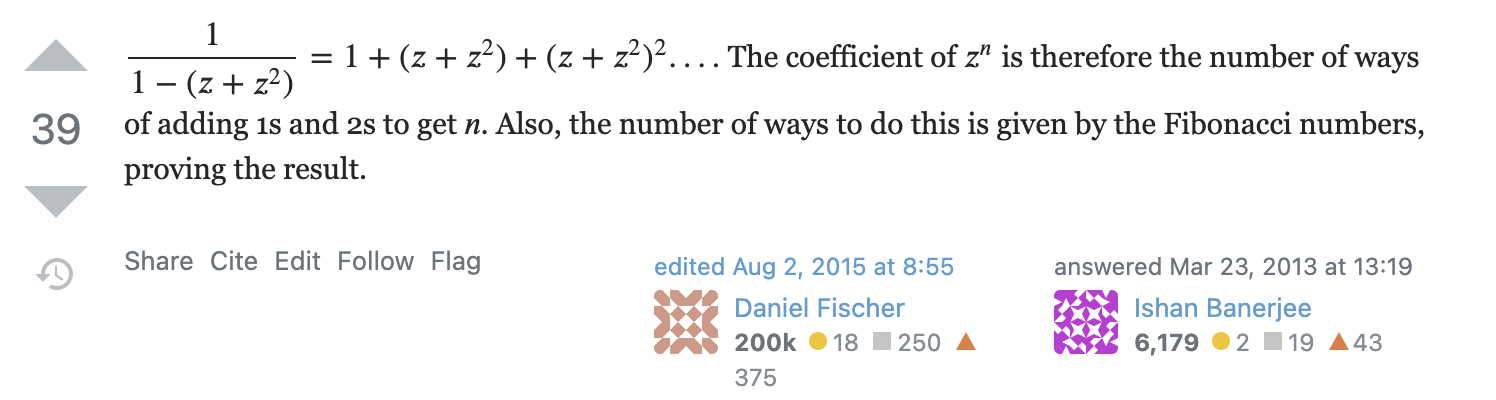
\includegraphics[width=400pt]{img/linear-algebra--vector-spaces-and-fields--computing-the-n-th-fibonacci-number-generating-function-d6da.png}
\end{mdframed}




\section{Finding the nth Fibonacci number via an eigenvector change of basis}


This problem is given at the end of the eigenvectors video in the Essence of Linear
Algebra\footnote{\url{https://www.youtube.com/playlist?list=PLZHQObOWTQDPD3MizzM2xVFitgF8hE_ab}} series by 3blue1brown\footnote{\url{http://www.3blue1brown.com/}}.


\subsection*{Introduction}

The Fibonacci sequence is the sequence you get by starting with $0, 1$ and after that always
forming the next number by adding the two previous ones: $0, 1, 1, 2, 3, 5, 8, 13, ...$.

Consider the matrix
\[
A = \matMMxNN{0}{1}
        {1}{1}
\]

The first few powers are

\begin{align*}
&A^{1} &= \matMMxNN{0}{1}
              {1}{1}
\\
&A^{2} = \matMMxNN{0}{1}
             {1}{1} \matMMxNN{0}{1}
                        {1}{1} &= \matMMxNN{1}{1}
                                      {1}{2}
\\
&A^{3} = \matMMxNN{0}{1}
             {1}{1} \matMMxNN{1}{1}
                        {1}{2} &= \matMMxNN{1}{2}
                                      {2}{3}
\\
&A^{4} = \matMMxNN{0}{1}
             {1}{1} \matMMxNN{1}{2}
                        {2}{3} &= \matMMxNN{2}{3}
                                      {3}{5}
\end{align*}

The matrix powers are generating the Fibonacci sequence:
\begin{align*}
  A^{n} = \matMMxNN{F_{n-1} }{F_n      }
  {F_n     }{F_{n+1} }
\end{align*}


So if there were a way to compute the $\nth$ power of that matrix ``directly'',
that would also be a way to compute the $\nth$ Fibonacci number ``directly'',
i.e. without computing all the preceding Fibonacci numbers \textit{en route}.

How can we do this? To state the problem in a different way, we need to
construct a new matrix that performs exactly the same transformation as $A^n$,
but which somehow does the exponentiation step ``in one go'' rather than by
multiplying $A$ with itself $n$ times.

\subsection*{Solution outline}

Matrices represent transformations, so we can talk about them as taking in some
vector and producing some other vector. The approach we're going to take is to
re-express the $A^n$ transformation as follows:

\begin{enumerate}
\item Convert the input vector to its representation in an alternative basis which uses the
  eigenvectors as the basis vectors (it's called an ``eigenbasis'').
\item In this alternative basis, compute the new position of the vector after carrying out the
  $A^n$ transformation.
\item Convert the resulting vector back to its representation in our original basis.
\end{enumerate}

I.e., we're going to compute the overall transformation as this product of
matrices (remember that one reads these things right-to-left):
\begin{align*}
  \begin{pmatrix}\text{matrix converting their}\\\text{representation to ours} \\ \end{pmatrix}
  \begin{pmatrix}\text{matrix that does the A transformation}\\\text{in the alternative basis} \\ \end{pmatrix}^n
  \begin{pmatrix}\text{matrix converting our}\\\text{representation to theirs} \\ \end{pmatrix}
\end{align*}
The crux of all this is that the exponentiation is efficient in the
eigenbasis. That's because, in the eigenbasis, the transformation is just
stretching space in the directions of the two basis vectors. So to do the
transformation $n$ times in the eigenbasis, you just stretch by the
stretch-factor raised to the $\nth$ power, rather than doing $n$ matrix
multiplications.

\subsection*{Solution details}

Let's suppose we've already found the eigenvectors, and that there are two of
them, and that we've arranged them as the two columns of a matrix $V$. $V$ holds
the basis vectors of the alternative basis, and therefore we know from the
[change of basis](\url{./linear-algebra.html#change-of-basis}) notes that $V$ is the
matrix that takes as input a vector expressed in the alternative basis and
outputs its representation in our basis.

So, step (3) is done by $V$, and step (1) is done by $V^{-1}$, and the matrix
performing all three steps is going to look like
\begin{align*}
  V
  \begin{pmatrix}\text{matrix that does the A transformation}\\\text{in the alternative basis} \\ \end{pmatrix}^n
  V^{-1}
\end{align*}
OK, so what is the matrix in the middle? The [change of
basis](\url{./linear-algebra.html#change-of-basis}) notes tell us that we can compute it as
\begin{align*}
  \begin{pmatrix}\text{matrix converting our}\\\text{representation to theirs} \\ \end{pmatrix}
  A
  \begin{pmatrix}\text{matrix converting their}\\\text{representation to ours} \\ \end{pmatrix}
\end{align*}
In other words the matrix in the middle is
\begin{align*}
  V^{-1}AV
\end{align*}
and the entire transformation is
\begin{align*}
  V
  \Big(V^{-1}AV\Big)^n
  V^{-1}
\end{align*}
Put back into words, that's
\begin{align*}
  \begin{pmatrix}\text{matrix converting their}\\\text{representation to ours} \\ \end{pmatrix}
  \Bigg(
  \begin{pmatrix}\text{matrix converting our}\\\text{representation to theirs} \\ \end{pmatrix}
  A
  \begin{pmatrix}\text{matrix converting their}\\\text{representation to ours} \\ \end{pmatrix}
  \Bigg)^n
  \begin{pmatrix}\text{matrix converting our}\\\text{representation to theirs} \\ \end{pmatrix}
\end{align*}

Recall that above we observed that the $\nth$ power of $A$ is a matrix with the
nth Fibonacci number in its bottom left and top right entries. So the following
tasks remain:
\begin{enumerate}
\item Find the eigenvectors and put them in a matrix $V$.
\item Find the inverse of $V$.
\item Compute the matrix product $V^{-1}AV$.
\item Compute the result of raising that to the $\nth$ power.
\item Plug the result of that into the overall expression.
\item Take the entry in the bottom left or top right (they should be the same!).
\end{enumerate}

The result should be an expression giving the $\nth$ Fibonacci number as a
function of $n$. It should be possible to give as input to that function the
number one million, and have it output the one millionth Fibonacci number
directly, without it having to go through the preceding 999,999 Fibonacci
numbers.


\subsection*{The answer without showing the calculations}

\begin{align*}
&\text{The eigenvectors are}
\\\\
&V &= \matMMxNN{2          }{2          }
        {1 + \sqrt 5}{1 - \sqrt 5}
\\\\
&\text{which has inverse}
\\\\
&V^{-1} &= \frac{-1}{4\sqrt 5} \matMMxNN{1 - \sqrt 5 }{-2}
                                 {-1 - \sqrt 5}{2}
\\\\
&\text{Therefore}
\\\\
&V^{-1}AV &= \frac{1}{2} \matMMxNN{1 + \sqrt 5}{0          }
                            {0          }{1 - \sqrt 5}
\\\\
&\text{and}
\\\\
&(V^{-1}AV)^n &= \frac{1}{2^n} \matMMxNN{(1 + \sqrt 5)^n}{0          }
                                   {0                }{(1 - \sqrt 5)^n}
\\\\
&\text{and}
\\\\
&V \Big(V^{-1}AV\Big)^n V^{-1} &=
\matMMxNN{\frac{\big((1 + \sqrt 5)^{n-1} - (1 - \sqrt 5)^{n-1}\big)}{2^{n-1}\sqrt 5}}{\frac{\big((1 + \sqrt 5)^n     - (1 - \sqrt 5)^n    \big)}{2^n    \sqrt 5}}
    {\frac{\big((1 + \sqrt 5)^n     - (1 - \sqrt 5)^n    \big)}{2^n    \sqrt 5}}{\frac{\big((1 + \sqrt 5)^{n+1} - (1 - \sqrt 5)^{n+1}\big)}{2^{n+1}\sqrt 5}}
\\\\
&\text{Therefore the nth Fibonacci number is}
\\\\
&F_n &= \frac{(1 + \sqrt 5)^n     - (1 - \sqrt 5)^n}
             {2^n    \sqrt 5}
\end{align*}

\newpage
\subsection*{Does this actually work?}

Yes.

\begin{minted}{python3}
    from math import sqrt

    def fib(n):
        return (
            ( (1 + sqrt(5))**n - (1 - sqrt(5))**n )
            /
            float(2**n * sqrt(5)))

    for i in range(10):
        print(i, fib(i))

    0 0.0
    1 1.0
    2 1.0
    3 2.0
    4 3.0
    5 5.0
    6 8.0
    7 13.0
    8 21.0
    9 34.0
\end{minted}

\subsection*{History}

The formula is known as
Binet's formula (\url{https://en.wikipedia.org/wiki/Fibonacci_number#Closed-form_expression})
(1843) but was apparently known to Euler, Daniel Bernoulli and de Moivre more
than a century earlier. It can be derived without using linear algebra
techniques; I don't know when the style of proof attempted here would first
have been done. The result can be written as

\begin{align*}
F_n = \frac{\varphi^n - \psi^n}{\sqrt{5}}
\end{align*}

where $\varphi = \frac{1+\sqrt{5}}{2}$ is the
golden ratio (\url{https://en.wikipedia.org/wiki/Golden_ratio}) and $\psi = 1 - \varphi = \frac{1 - \sqrt{5}}{2}$.


\subsection*{Calculations}

\subsubsection{1. Find the eigenvectors}
We have

\begin{align*}
A = \matMMxNN{0}{1}
        {1}{1}.
\end{align*}
An eigenvector $v$ satisfies $Av = \lambda v$ for some scalar $\lambda$. That
equation can be rearranged as follows

\begin{align*}
A\vec v &= \lambda I\vec v
\\
A\vec v - \lambda I\vec v &= \vec 0
\\
(A - \lambda I)\vec v &= \vec 0
\end{align*}

which means that the matrix $A - \lambda I$ is a transformation that takes some
non-zero vector $\vec v$ to the zero vector (i.e. it has a non-empty ``null
space''). This means that the transformation cannot be reversed, i.e. the matrix
has no inverse, i.e. its determinant is zero. So, use that last fact to find
the eigenvectors $\lambda$:

\begin{align*}
\det (A - \lambda I) &= 0
\\
\\
\det \matMMxNN{-\lambda}{1}
         {1          }{1 - \lambda} &= 0
% \\
% \\
% (-\lambda)(1 - \lambda) - 1 &= 0
\\
\\
\lambda^2 - \lambda - 1 = 0
\end{align*}

Using the quadratic formula we have $a=1, b=-1, c=-1$ and

\begin{align*}
\lambda
= \frac{-b \pm \sqrt{b^2 - 4ac}}{2a}
= \frac{1 \pm \sqrt{5}}{2}
\end{align*}

which are the two eigenvalues: $\varphi$ and $\psi$.

To find eigenvectors associated with the eigenvalues, go back to the equations

\begin{align*}
(A - \lambda I)\vec v &= \vec 0
\\
\\
\matMMxNN{-\lambda}{1}
    {1       }{1 - \lambda} \vec v &= \vec 0
\end{align*}

Let an eigenvector $v$ be $\scvec{v_1}{v_2}$. The matrix equation corresponds
to this system of equations:

\begin{align*}
\begin{cases}
-\lambda v_1 + v_2               &= 0\\
v_1          + (1 - \lambda) v_2 &= 0
\end{cases}
\end{align*}

From the first equation we have $v_2 = \lambda v_1$. There are infinitely many
eigenvectors (a line of them) associated with any given eigenvalue, so we can
pick an arbitrary value for $v_1$. If we choose $v_1 = 1$ then we have
eigenvectors $\scvec{1}{\varphi}$ and $\scvec{1}{\psi}$. The matrix
containing the eigenvectors is

\begin{align*}
V = \matMMxNN{1}{1}
             {\varphi}{\psi}
\end{align*}

\subsubsection{2. Find inverse of $V$}


The inverse of a 2x2 matrix is given by
\begin{align*}
\matMMxNN{a}{c}
    {b}{d} ^ {-1}
=
\frac{1}{\text{det}} \matMMxNN{d}{-c}
                         {-b}{a}
\end{align*}
where $\text{det} = ad - cb$. We have $\varphi - \psi = \sqrt5$ therefore
\begin{align*}
V^{-1}
&= \frac{-1}{\sqrt5} \matMMxNN{\psi}{-1}
                          {-\phi}{1}
\end{align*}


\subsubsection{3. Find the matrix product $V^{-1}AV$

Before getting lost in calculations, let's remember what this is. It's a
matrix that does the $A$ transformation, but \textit{in the coordinate system defined
by $A$'s eigenvectors}. So, the resulting matrix \textit{must} do nothing other than
stretch space in the direction of one or both basis vectors in that coordinate
system. That's because (1) we represent a transformation with a matrix saying
where each of the basis vectors are taken to, (2) the definition of an
eigenvector of a transformation is that it is a vector which is simply
stretched by the transformation with no change in direction, therefore (3) if
the eigenvectors are the basis vectors, then the matrix representing the
transformation must just stretch space in the two directions. A matrix which
stretches space in the direction of the basis vectors looks like
$\smat{a}{0}{0}{b}$, i.e. it is diagonal. Therefore, $V^{-1}AV$ \textit{must} be
diagonal.

\begin{align*}
V^{-1}AV &=
\frac{1}{\sqrt5}
\matMMxNN{-\psi}{1}
         {\phi }{-1}
\matMMxNN{0}{1}
         {1}{1}
\matMMxNN{1}{1}
         {\varphi}{\psi}
\\\\
&=
\frac{1}{\sqrt5}
\matMMxNN{-\psi}{1 }
         {\varphi }{-1}
\matMMxNN{\varphi    }{\psi    }
         {1 + \varphi}{1 + \psi}
\\\\
&=
\frac{1}{\sqrt5}
\matMMxNN{-\varphi\psi + (1 + \varphi)}{-\psi^2 + (1 + \psi)}
         {\varphi^2 - (1 + \varphi)}{\varphi\psi - (1 + \psi)}
\\\\
&=
\frac{1}{\sqrt5}
\matMMxNN{\varphi}{0}
         {0}{-\psi}
\end{align*}

Where we have used $\varphi\psi = 1$, and $\varphi^2 = 1 + \varphi$, and $\psi^2 = 1 + \psi$.



\subsubsection{4. Compute $(V^{-1}AV)^n$}

The matrix is diagonal so this is straightforward:

\begin{align*}
(V^{-1}AV)^n = \frac{1}{\sqrt{5}^n} \matMMxNN{\varphi^n}{0    }
                                       {0 }{(-\psi)^n}
\end{align*}

Note that this is the whole point of converting to the eigenbasis: the exponentiation at this step
just involves the usual operations of raising scalar numbers to a power; no need to multiply
matrices together. A computer will be able to compute the $\nth$ power of a diagonal matrix much
faster than that of a non-diagonal matrix.



\subsubsection{5. Plug the $\nth$ power into the overall expression}

\begin{align*}
V \Big(V^{-1}AV\Big)^n V^{-1}
&=
\frac{-1}{4\sqrt 5}
\frac{1}{2^n}
\matMMxNN{2          }{2          }
    {1 + \sqrt 5}{1 - \sqrt 5}
\matMMxNN{(1 + \sqrt 5)^n}{0              }
    {0              }{(1 - \sqrt 5)^n}
\matMMxNN{1 - \sqrt 5 }{-2}
    {-(1 + \sqrt 5)}{2}
\\\\
&=
\frac{-1}{4\sqrt 5}
\frac{1}{2^n}
\matMMxNN{2          }{2          }
    {1 + \sqrt 5}{1 - \sqrt 5}
\matMMxNN{(1 - \sqrt 5)(1 + \sqrt 5)^n}{-2(1 + \sqrt 5)^n}
    {-(1 + \sqrt 5)(1 - \sqrt 5)^n}{2(1 - \sqrt 5)^n}
\\\\
&=
\frac{-1}{4\sqrt 5}
\frac{1}{2^n}
\matMMxNN{2(-4)\big((1 + \sqrt 5)^{n-1} - (1 - \sqrt 5)^{n-1}\big)}{-4\big((1 + \sqrt 5)^n     - (1 - \sqrt 5)^n    \big)}
    {   -4\big((1 + \sqrt 5)^n     - (1 - \sqrt 5)^n    \big)}{-2\big((1 + \sqrt 5)^{n+1} - (1 - \sqrt 5)^{n+1}\big)}
\\\\
&=
\frac{1}{4\sqrt 5}
\matMMxNN{4\frac{\big((1 + \sqrt 5)^{n-1} - (1 - \sqrt 5)^{n-1}\big)}{2^{n-1}}}{4\frac{\big((1 + \sqrt 5)^n     - (1 - \sqrt 5)^n    \big)}{2^n    }}
    {4\frac{\big((1 + \sqrt 5)^n     - (1 - \sqrt 5)^n    \big)}{2^n    }}{ \frac{\big((1 + \sqrt 5)^{n+1} - (1 - \sqrt 5)^{n+1}\big)}{2^{n-1}}}
\\\\
&=
\matMMxNN{\frac{\big((1 + \sqrt 5)^{n-1} - (1 - \sqrt 5)^{n-1}\big)}{2^{n-1}\sqrt 5}}{\frac{\big((1 + \sqrt 5)^n     - (1 - \sqrt 5)^n    \big)}{2^n    \sqrt 5}}
    {\frac{\big((1 + \sqrt 5)^n     - (1 - \sqrt 5)^n    \big)}{2^n    \sqrt 5}}{\frac{\big((1 + \sqrt 5)^{n+1} - (1 - \sqrt 5)^{n+1}\big)}{2^{n+1}\sqrt 5}}
\end{align*}


\newpage
\section{Polynomials, rings, minimal and characteristic polynomials}

Let $f(x) \in \F[x]$ be a polynomial: $f(x) = a_kx^k + \ldots + a_0$.

Let $A \in M_n(\F)$ be an $n \times n$ matrix over a field $\F$.

We can evaluate the polynomial on the matrix: $f(A) = a_kA^k + \ldots + a_0I$.

\begin{theorem*}
  For all $A \in M_n(\F)$, there exists $f(x) \in \F[x]$ such that $f(A) = 0$.
\end{theorem*}

\begin{proof}
  Note that $\dim M_n(\F) = n^2$.\footnote{Let $\Delta_{ij} \in M_n(\F)$ be the matrix with $(i,j)$-th entry 1, and 0
    elsewhere. Then $\{\Delta_{ij} ~|~ i,j \leq n\}$ is a basis.}

  Let $k > n^2$. Then $A^k, A^{k-1}, \ldots, I$ is linearly dependent. Therefore there exists a
  $k$-th degree polynomial $f(x) \in \F[x]$ such that $f(A) = 0$.
\end{proof}

\begin{theorem*}
  The assignment $E_A: f(x) \to f(A)$ is a ring homomorphism.
\end{theorem*}

\red{It's not an isomorphism because some $f(A) = g(A)$ for $f \neq g$? I.e. it's non-injective.
  So the kernel is the set of polynomials $p(x)$ such that $p(A) = 0$. It contains the minimal and
  characteristic polynomials.}

\begin{proof}
  Let $f, g \in \F[x]$ with $f(x) = a_Jx^J + \ldots + a_0$ and $g(x) = b_Jx^J + \ldots + b_0$. (If
  $f$ and $g$ are not of the same degree then pad the lower degree one with zero coefficients to
  make it the same degree as the higher one.)

  Addition:
  \begin{align*}
    E_A\Big((f + g)(x)\Big) &= (f + g)(A)\\
                            &= f(A) + g(A)~~~~\text{(by definition of addition of polynomials)}\\
                            &= E_A\Big(f(x)\Big) + E_A\Big(g(x)\Big)
  \end{align*}
  Multiplication:
  \begin{align*}
    E_A\Big((fg)(x)\Big)    &= (fg)(A)\\
                            &= f(A)g(A)~~~~\text{(by definition of multiplication of polynomials)}\\
                            &= E_A\Big(f(x)\Big)E_A\Big(g(x)\Big)
  \end{align*}
\end{proof}

\begin{definition*}[Minimal polynomial]
  Let $V$ be a finite-dimensional vector space over $\F$, and let $A$ be a matrix of a linear
  transformation $T:V \to V$.

  The \emph{minimal polynomial} $m_A(x)$ is the monic polynomial $p(x)$ of minimal degree such that
  $p(A) = 0$.
\end{definition*}

\begin{theorem*}
  ~\\
  \begin{enumerate}
  \item The minimal polynomial is unique.
  \item Let $f(x)$ be a polynomial. If $f(A) = 0$ then $m_A | f$.
  \end{enumerate}
\end{theorem*}


\section{Quotient spaces, induced maps}

\begin{theorem*}
  Let $T:V \to W$ be an isomorphism\footnote{note: not linear; but why not homomorphism?} between
  vector spaces $V$ and $W$, and let $A \subseteq V, B \subseteq W$ be subspaces. Then the formula
  $\bar T(v + A) = T(v) + B$ gives a well-defined linear map $\bar T:V/A \to W/B$ if and only if
  $T(A) \subseteq B$.
\end{theorem*}

Therefore

\begin{theorem*}
  Let $T:V \to V$ with $U$ a subspace of $V$. If $U$ is $T$-invariant, then $T$ induces a linear
  map of quotients $\bar T:V/U \to V/U$ given by $v + U \mapsto T(v) + U$.
\end{theorem*}
\section{Cross product}
\begin{definition*}
  The cross product is defined for 3-dimensional vectors only. It can be written as a formal
  determinant
  \begin{align*}
    u \times v = \Bigg|
    \vmatMMMxNNN
    {\mathbf{i}}{\mathbf{j}}{\mathbf{k}}
    {u_1}{u_2}{u_3}
    {v_1}{v_2}{v_3}
    \Bigg|,
  \end{align*}
  which can be computed using the cofactor expansion:
  \begin{align*}
    u \times v =
      (u_2v_3 - u_3v_2)\mathbf{i}
    - (u_1v_3 - u_3v_1)\mathbf{j}
    + (u_1v_2 - u_2v_1)\mathbf{k}.
  \end{align*}
\end{definition*}


\section{Singular Value Decomposition}
\footnotetext{Notes from Kun (2018) A Programmer's Introduction to Mathematics}

% https://news.ycombinator.com/item?id=19014932

% After teaching Linear Algebra, here's my litmus test for a good book. At a glance, it should make the following clear first and foremost:

% 1. A matrix of a linear map F is simply writing down the image of the standard basis F(e_1),
% F(e_2), ... F(e_n). These vectors are the columns of the matrix. If you know them, you can compute
% F(v) for any v by linearity. That's called "multiplying a vector by matrix"; we write Mv = F(v).

% 2. The product of matrices is simply the matrix of composition of linear maps that they
% represent. The student can figure out what that matrix should be (or should be able to do so);
% here's how. If M is the matrix of F, and N is the matrix of G (where F and G are linear maps), then
% the first column of MN is F(G(e_1)) = M x (first column of N). Same for other columns. Ta-dah.

% 3. The determinant of v_1, .. v_n is simply the volume of the lopsided box formed by these vectors
% (mathematicians call the box "parallelepiped"). In particular, in a plane, the area of the triangle
% formed by vectors A and B is half the determinant. This are can have a minus sign; switching any
% pair of vectors flips the sign.

% 4. Eigenvectors and eigenvalues are fancy words that allow us to describe linear maps like this:
% "Stretch this picture along these directions by this much". Directions are eigenvectors, by how
% much - eigenvalues.

% Bonus:

% 5. Rotation and scaling are linear maps. That's all any linear map does: rotates and
% stretches. Writing a map down in this way is called singular value decomposition.

% 6. Shears are linear maps that don't change the volume. Any box can be made rectangular by applying
% a bunch of shears to it. That's called Gaussian elimination or row reduction when you look at what
% happens to matrices (and apply scaling as the last step). This is also an explanation of why the
% determinant gives volume (if you define it as an alternating n-linear form).



There is a problem when learning to study university-level mathematics. Away from the world of
technical literature, we are familiar with ``reading'': it involves quickly looking at and
comprehending one sentence after another until you've finished the page, and then turning the
page. However in mathematics, books and lecture notes are written as a large collection of
definition-theorem-proof sequences, interspersed with fairly terse discussion, and the material
progresses much too rapidly to be read in the usual way.

In fact, this stuff cannot be read purely in passive mode.  What you need to do is read the
definition a few times, and then stop and write down a list of concrete examples of the thing being
defined. Then read the theorem a few times, and try to convince yourself that it holds for each of
your examples. And then find a time at which you have the mental energy and disposition to study
and fully understand the proof.

However. There {\it is} an important part of studying mathematics that doesn't require actually
being at a table for hours with writing materials or computer at hand. That part involves thinking
hard about important bits. It can be done on public transport. It can be done in bed. It involves
thinking the thing over until it becomes genuinely familiar; confronting and reconciling different
perspectives, confronting and eliminating remaining areas of muddled thinking.

What is needed is a helping hand in the form of suitable reading material. Books of prayer and
meditation have been around for a while.  The purpose here is not to develop an entire area of
mathematical theory in a logical, organised fashion; the purpose is to become good at thinking
about certain small but important areas. While we will define things carefully, unlike the standard
mathematical literature we're going to state theorems informally without proof, and partially
repeat ourselves again and again while retreading the same ground in a slightly different
direction.

We'll start with an area that we will keep small and that no-one is going to dispute is important:
...

% the basic ideas of vector space, basis, linear transformation, and matrix multiplication.

% This section makes use of the following concepts.
% \begin{enumerate}
% \item {\it Vector space}: A vector space is a set of vectors. Key basic examples are
%   \begin{enumerate}
%   \item An infinite straight line passing through an origin point. Every point on the line is a
%     one-dimensional vector.
%   \item 3-dimensional Euclidean space with an origin point. This is referred to as $\R^3$.
%   \end{enumerate}
% \item {\it basis}: A basis is a minimal set of vectors that span a vector space. In $\R^3$ it is
%   essentially the same as the concept of ``coordinate axes''. Note however that someone could force
%   you to use coordinate axes that are not orthogonal to each other. That would still work for
%   specifying locations unambiguously, although it might be a bit inconvenient. The same things
%   holds for the set of vectors making up a basis: they just have to span the space; they need not
%   be orthogonal to each other.
% \end{enumerate}

\newpage
\subsection*{The data, viewed as vectors}

3 people rate 8 films. We write the data as a matrix:
\begin{align*}
\bordermatrix{
                &\text{Person 1} & \text{Person 2} &\text{Person 3} \cr
  \text{Film 1} &3               &  2              &  5             \cr
  \text{Film 2} &3               &  4              &  3             \cr
  \text{Film 3} &2               &  3              &  1             \cr
  \text{Film 4} &4               &  5              &  4             \cr
  \text{Film 5} &1               &  2              &  3             \cr
  \text{Film 6} &3               &  1              &  5             \cr
  \text{Film 7} &1               &  3              &  5             \cr
  \text{Film 8} &2               &  5              &  1             \cr
}
\end{align*}

\begin{tabular}{|p{8cm}|p{8 cm}|}
  {\bf The column view}
  &{\bf The row view}\\

  \hline
  &\\
  We think of this matrix as 3 columns.
  &We think of this matrix as 8 rows.\\
  &\\

  Focus on column 1: it contains ratings for all the films, from Person 1.
  &Focus on row 1: it contains ratings from all the people, for Film 1.\\
  &\\

  The column is a vector in $\R^8$: its coordinates are $(3,3,2,4,1,3,1,2)$ with respect to the basis. What is the
  basis?
  &The row is a vector in $\R^3$: its coordinates are $(3, 2, 5)$ with respect to the basis. What is the
    basis?\\
  &\\

  Writing the data with one row per film implicitly specified the basis for $\R^8$:
  it consists of 8 orthogonal vectors, each corresponding to a single one of the 8 films.
  &Writing the data with one column per person implicitly specified the basis for $\R^3$:
    it consists of 3 orthogonal vectors, each corresponding to a single one of the 3 people.\\
  &\\

  For example, one of the basis vectors is $(0, 1, 0, 0, 0, 0, 0, 0)$. This is the
  vector representation of Film 2.
  &For example, one of the basis vectors is $(0, 1, 0)$. This is the vector
    representation of Person 2.\\
  &\\

  The basis is\\ $\{(1, 0, 0, 0, 0, 0, 0, 0), (0, 1, 0, 0, 0, 0, 0, 0), \ldots\}$.
  &The basis is $\{(1, 0, 0), (0, 1, 0), (0, 0, 1)\}$.\\
  &\\

  Column 1 is a vector with coordinates $(3,3,2,4,1,3,1,2)$.
  It represents a film: an imaginary film that is a linear combination of the 8 real
  films represented by the 8 basis vectors.
  &Row 1 is a vector with coordinates $(3, 2, 5)$.
    It represents a person: an imaginary person that is a linear combination of the 3 real
    people represented by the 3 basis vectors.\\
  &\\

  This is despite the fact that the column is labeled ``Person 1'': the column vector represents a film, not a person.
  &This is despite the fact that the row is labeled ``Film 1'': the row vector represents a person, not a film.\\
  &\\

  Column 1 is a linear combination of the 8 films: it is
  $(3 \times \text{Film 1}) + (3 \times \text{Film 2}) + \ldots$
  &Row 1 is a linear combination of the 3 people: it is
    $(3 \times \text{Person 1}) + (2 \times \text{Person 2}) + (5 \times \text{Person 3})$\\
  &\\

  The data are 3 vectors (aka points) in $\R^8$.
  &The data are 8 vectors (aka points) in $\R^3$.
\end{tabular}

Whenever we specify the coordinates of a vector in any vector space, we are specifying a linear
combination of the basis vectors.

\newpage
\subsection*{The data, viewed as a linear transformation}

3 people rate 8 films. We write the data as a matrix:
\begin{align*}
\bordermatrix{
                &\text{Person 1} & \text{Person 2} &\text{Person 3} \cr
  \text{Film 1} &3               &  2              &  5             \cr
  \text{Film 2} &3               &  4              &  3             \cr
  \text{Film 3} &2               &  3              &  1             \cr
  \text{Film 4} &4               &  5              &  4             \cr
  \text{Film 5} &1               &  2              &  3             \cr
  \text{Film 6} &3               &  1              &  5             \cr
  \text{Film 7} &1               &  3              &  5             \cr
  \text{Film 8} &2               &  5              &  1             \cr
}
\end{align*}
\begin{tabular}{|p{8cm}|p{8 cm}|}
  {\bf The column view}
  &{\bf The row view}\\

  \hline
  &\\
  The data matrix represents a function $f: \R^3 \to \R^8$.
  &The data matrix represents a function $g: \R^8 \to \R^3$.\\
  &\\

  $f$ is a function from person-space (3-dimensional) to film-space (8-dimensional).
  &$g$ is a function from film-space (8-dimensional) to person-space (3-dimensional).\\
  &\\

  Focus on Person 1, who is represented by $(1, 0, 0)$.
  &Focus on Film 1, which is represented by $(1, 0, 0, 0, 0, 0, 0, 0)$.\\
  &\\

  $f$ maps Person 1 to an imaginary film in film-space.
  &$g$ maps Film 1 to an imaginary person in person-space.\\
  &\\

  $f$ maps Person 1 to the vector of film ratings made by Person 1.
  &$g$ maps Film 1 to the vector of ratings of Film 1 made by the 3 people.\\
  &\\

  $f$ is a linear model for the data-generation process. It says that to generate the film ratings for a new person $x$:
  \begin{enumerate}
  \item First determine $x$'s coordinates in person-space as a combination of the original 3 people.
  \item Then
  \end{enumerate}

  To where does $f$ map row 1? \red{nowhere interesting?}
  &To where does $g$ map column 1? \red{nowhere interesting?}
\end{tabular}

\newpage
The matrix is 3 vectors in $\R^8$. Each vector is a linear combination of the 8 real films

\subsection*{Linear map}

As an $8 \times 3$ matrix, this represents a linear map $\R^3 \to \R^8$.

This map is (person-space) $\to$ (film space).

The domain (person-space) is a 3-dimensional vector space. The 3 vectors in the basis for this
space are the 3 people: $\{(1, 0, 0), (0, 1, 0), (0, 0, 1)\}$. Points in the space represent linear
combinations of people.

The codomain (film-space) is an 8-dimensional vector space. The 8 vectors in the basis for this
space are the 8 films. Points in the space represent linear combinations of films.

Thus writing the data in a matrix implies that we are specifying a {\it linear model} that
describes the {\it process} of rating a film: the model specifies a linear map that takes a person
as input and outputs their ratings.

(We could also view the model as being the transpose: taking a vector of ratings as input and
outputting a person who would give those ratings.)

Thus we assume
\begin{enumerate}
\item The model is the same for all people.
\item $f(\alpha p_1 + \beta p_2) = \alpha f(p_1) + \beta f(p_2)$: the ratings for a
  linear-combination person are given by forming the same linear combination of ratings of the
 combination.
\end{enumerate}
